%%%%%%%%%%%%%%%%%%%%%%%%%%%%%%%%%%%%%%%%%%%%%%%%%%%%%%%%%%%%%%%
%
% Welcome to Overleaf --- just edit your LaTeX on the left,
% and we'll compile it for you on the right. If you open the
% 'Share' menu, you can invite other users to edit at the same
% time. See www.overleaf.com/learn for more info. Enjoy!
%
%%%%%%%%%%%%%%%%%%%%%%%%%%%%%%%%%%%%%%%%%%%%%%%%%%%%%%%%%%%%%%%
% -------------------------------------------------------------------------------
% This is all preamble stuff that you don't have to worry about.
% Head down to where it says "Enter your name here"
% -------------------------------------------------------------------------------
 
\documentclass[12pt]{article}
 
\usepackage[margin=1in]{geometry} 
\usepackage{amsmath,amsthm,amssymb}
\usepackage{graphicx}
\usepackage{enumerate}
\usepackage[names]{xcolor}
\usepackage[multiple,hang,flushmargin]{footmisc}
\usepackage{lastpage}
\usepackage{tikz}
\usepackage{listings}
\usepackage[parfill]{parskip}
\parskip=\baselineskip

 
\newenvironment{question}[2][Question]{\begin{trivlist}
\item[\hskip \labelsep {\bfseries #1}\hskip \labelsep {\bfseries #2.}]}{\end{trivlist}}
\newenvironment{solution}[1][Solution:]{\begin{trivlist}
\item[\hskip \labelsep {\bfseries #1}\hskip \labelsep {\bfseries}]\color{blue}}{\end{trivlist}}

\usepackage{fancyhdr}
\pagestyle{fancy}
\rhead{Due: \duedate}
\lhead{CSC250 - Midterm}
\cfoot{p. \thepage \ of \pageref{LastPage}}
\renewcommand{\headrulewidth}{0.4pt}
\renewcommand{\footrulewidth}{0.4pt}

 
\begin{document}
\newcommand{\duedate}{11:59PM EST Thursday October 24, 2024}
 

% --------------------------------------------------------------------------------------------
%  Great, now skip ahead to where you see *** START EXAM HERE ***
% --------------------------------------------------------------------------------------------

\topskip0pt
\vspace*{\fill}
\begin{center}
\fbox{\fbox{\parbox{5.5in}{\begin{center}
\vspace{1em}
This is the first of two examinations for\\ \textbf{CSC250: Theory of Computation}\\ as taught by Pablo Frank Bolton in Fall 2024.\\
\vspace{1em}
This exam is \textbf{open book and open note}.\\ The following materials are \textbf{permitted} while taking this examination:
\vspace{1em}
\begin{itemize}
	\item your own notes
	\item lecture slides / videos
	\item scribe notes
	\item homework solutions
	\item any of the recommended textbooks
\end{itemize}
\vspace{1em}
\textbf{Honor code: no other resources are permitted during this exam.}\\
This includes (but is not limited to): online materials, tutors, teaching assistants, and other students.
\end{center}
\vspace{5em}
 \ \ \ YOUR NAME: \underline{\hspace{10cm}}
\vspace{3em}}}}
\end{center}
\vspace{3em}
\vspace*{\fill}


% ---------------------------------------
%   *** START EXAM HERE ***
% ---------------------------------------

\clearpage
\begin{question}{0}\textbf{Getting in the Groove} (0 points)
\begin{center}
\textit{Note: This question is optional, but strongly recommended.}
\end{center}
Educational research studies\footnote{\scriptsize{Lang, Jonas WB, and Jessica Lang. ``Priming competence diminishes the link between cognitive test anxiety and test performance: Implications for the interpretation of test scores.'' \textit{Psychological Science} 21.6 (2010): 811-819.}}\footnote{\scriptsize{Barrows, Jennifer, Samantha Dunn, and Carrie A. Lloyd. ``Anxiety, self-efficacy, and college exam grades.'' \textit{Universal Journal of Educational Research} 1.3 (2013): 204-208.}} have suggested that people perform better on tests when they spend a few minutes thinking about things they're good at before they begin.\\\\
In the space below, briefly tell us about a time when you were \textbf{really successful} at doing something challenging (it doesn't have to be related to this course). If you prefer, you can draw a picture instead of writing.\\
\vfill
\hfill
% 
\includegraphics[width=2in]{youcandoit.png}
\end{question}

% --------
% Logic
% --------
%\clearpage
%\begin{question}{1}\textbf{Propositional logic}\\\\
%Consider the following propositions:
%\begin{eqnarray*}
%	p & = & \texttt{It was raining.}\\
%	q & = & \texttt{We played board games inside.}\\
%	r & = & \texttt{We went to the beach.}
%\end{eqnarray*}
%Translate each of the following propositions into an English sentence.
%\begin{enumerate}[(a)]	
%	\item $q \vee r$\vspace{8em}
%	\item $p \rightarrow q$\vspace{8em}
%	\item $q \rightarrow \neg r$\vspace{8em}
%	\item $p \wedge \neg r \rightarrow q$
%\end{enumerate}
%\end{question}
%
\clearpage
\begin{question}{1}\textbf{Valid or Invalid Reasoning} (6 points)\\\\
For each of the following English arguments, express the argument in terms of
propositional logic and briefly justify whether the argument is valid or invalid. Be sure to clearly label your propositions.
\begin{enumerate}[(a)]	
	\item \textit{When the weather is nice, Max either rides their bike on the rail trail or goes for a walk through the gardens (but never both on the same day). The weather is nice, and Max is going for a walk through the gardens. Therefore, Max will not ride their bike on the rail trail today.}

    \begin{solution}
        \begin{align*}
        &N : \text{Weather is \textbf{N}ice} \\
        &B : \text{Max rides a \textbf{B}ike} \\
        &W : \text{Max takes a \textbf{W}alk} \\
        &N \rightarrow B \oplus W \\
        &N : True \\
        &W : True \\
        \end{align*}
        Conclusion to check: "Max will NOT ride a bike today"
        or $B : False$

        We can express the information in the following table:
        
\begin{table}[h!]
\centering
\begin{tabular}{|l|l|l|l|l|}
\hline
N & B & W & B $\oplus$ W & N $\rightarrow B \oplus W$ \\ \hline
1 & 0 & 1 & 1                         & 1                                                      \\ \hline
1 & 1 & 1 & 0                         & 0                                                      \\ \hline
\end{tabular}
\end{table}        
        As it can be seen, if Max goes on a bike ride (second row), the implication does not hold, so B: False must be the case (first row) and the conclusion is \textbf{valid}.
    \end{solution}
    
 
	\item \textit{When a student needs a book and a coffee,  they go to Neilson Library. There is a student at Neilson Library today. This means that they wanted to check out a book.}
    \begin{solution}
        \begin{align*}
        &B : \text{Student wants to check out a \textbf{B}ook} \\
        &C : \text{Student wants a \textbf{C}offee} \\
        &N : \text{Students go to \textbf{N}ielson} \\
        &B \cap C \rightarrow N \\
        &N : True \\
        \end{align*}

        Conclusion to check: "The student wanted to check out a book"
        or $B : True$

        We can express the information in the following table:

\begin{table}[h!]
\begin{tabular}{|l|l|l|l|l|}
\hline
B & C & B $\cap$ C & N & B $\cap$ C $\rightarrow$ N \\ \hline
0 & 0 & 0                       & 1 & 1                              \\ \hline
0 & 1 & 0                       & 1 & 1                              \\ \hline
1 & 0 & 0                       & 1 & 1                              \\ \hline
1 & 1 & 1                       & 1 & 1                              \\ \hline
\end{tabular}
\end{table}

% \begin{table}[h!]
% \centering
% \begin{tabular}{|l|l|l|}
% \hline
% N & B & $N\rightarrow B$ \\ \hline
% 0 & 0 & 1               \\ \hline
% 0 & 1 & 1               \\ \hline
% 1 & 0 & 0               \\ \hline
% 1 & 1 & 1               \\ \hline
% \end{tabular}
% \end{table}

        The first point is that the implication must be B $\cap$ C $\rightarrow$ N. Since the conclusion of the implication is always true: $N:True$, any value for the condition will make the implication hold. It is possible that a student is at Nielson for any reason, where two cases do not involve wanting to get a book... so the conclusion is \textbf{invalid}  
    \end{solution}
    
\end{enumerate}
\end{question}

% ---------------------------
% Regular expressions
% ---------------------------
\clearpage
\begin{question}{2}\textbf{Interpreting regular expressions} (3 points)\\\\
Describe the language matched by the following regular expression:
\[ (0 + 10 )^*\]
Note: Try to describe the resulting language, not the regular expression.
\end{question}

\begin{solution}
\;

    \textbf{Option 1:} This is the language of binary words where any 1 must be followed by at least one zero.
\end{solution}

\begin{question}{3}\textbf{Writing regular expressions} (3 points)\\\\
Consider the following language on the alphabet $\Sigma = \{0,1\}$:
\[L = \{w \ | \ w \texttt{ has even length, and starts and ends with the same symbol}\}\]
Write a regular expression for $L$.
\end{question}

\begin{solution}
$0(\Sigma\Sigma)^*0 + 1(\Sigma\Sigma)^*1$
\end{solution}

% ----------------------
% Finite automata
% ----------------------
\clearpage
\begin{question}{4}\textbf{Interpreting  Finite Automata} (4 points)\\\\
Consider the following finite automaton:
\begin{center}
	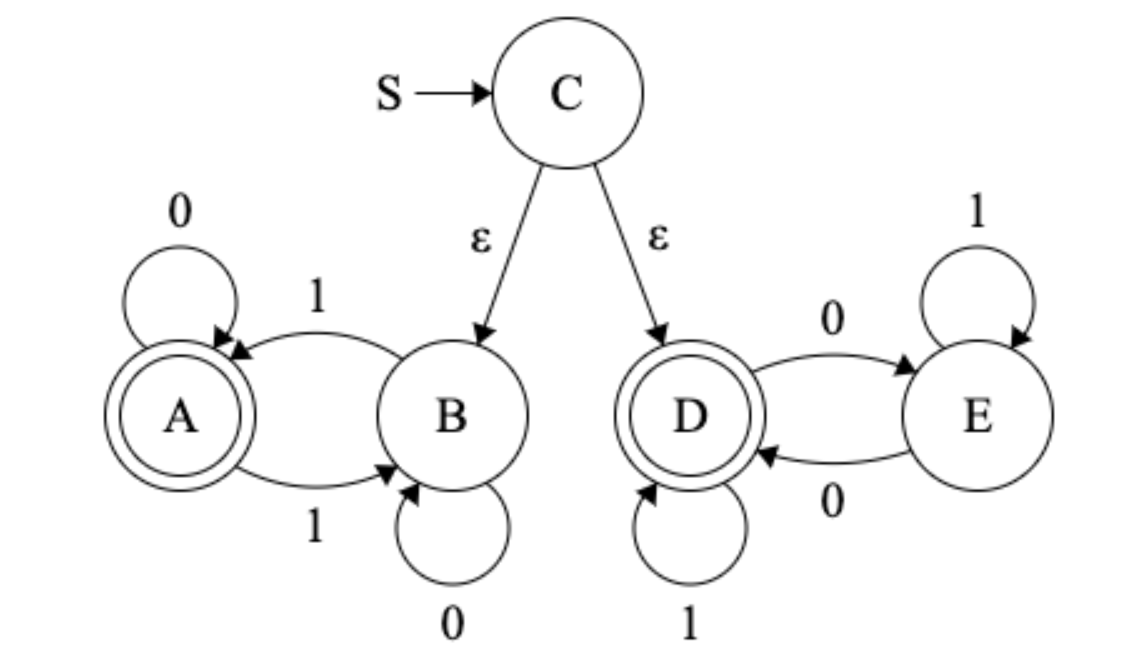
\includegraphics[width=0.6\textwidth]{q4-FA.png}
\end{center}
\begin{enumerate}[(a)]
    \item What is the start state?
        \begin{solution}
            $C$
        \end{solution}
	\item What is the set of accepting states?
        \begin{solution}
            $\{A, D\}$
        \end{solution}
	\item Is this a DFA, an NFA, neither, or both?
        \begin{solution}
            This is an NFA with $\epsilon$-jumps (so it has NFA-properties).
        \end{solution} 
	\item What is the language accepted by this FA?
        \begin{solution}
            $L = \{ w \in \Sigma^* \vert \text{w either an even number of zeros or an odd number of ones} \}$
        \end{solution}  
	
\end{enumerate}
\end{question}

\clearpage
\begin{question}{5}\textbf{Building Finite Automata} (6 points)\\\\
Draw the transition diagram for a finite automaton that recognizes each of the following languages. In all cases, the alphabet is $\Sigma = \{0,1\}$.
\begin{enumerate}[(a)]
	\item $\{ w \in \Sigma^* \ | \ w \texttt{ begins with } 1 \texttt{ and ends with } 0 \}$.
\begin{solution}
\;

\begin{center}
\begin{tikzpicture}[scale=0.2]
\tikzstyle{every node}+=[inner sep=0pt]
\draw [black] (13.3,-25.2) circle (3);
\draw (13.3,-25.2) node {$A$};
\draw [black] (23.4,-25.2) circle (3);
\draw (23.4,-25.2) node {$B$};
\draw [black] (33.6,-25.2) circle (3);
\draw (33.6,-25.2) node {$C$};
\draw [black] (33.6,-25.2) circle (2.4);
\draw [black] (45.6,-25.1) circle (3);
\draw (45.6,-25.1) node {$A$};
\draw [black] (54.8,-25.1) circle (3);
\draw (54.8,-25.1) node {$B$};
\draw [black] (64,-25.1) circle (3);
\draw (64,-25.1) node {$C$};
\draw [black] (64,-25.1) circle (2.4);
\draw [black] (13.3,-19.9) -- (13.3,-22.2);
\draw (13.3,-19.4) node [above] {$S$};
\fill [black] (13.3,-22.2) -- (13.8,-21.4) -- (12.8,-21.4);
\draw [black] (16.3,-25.2) -- (20.4,-25.2);
\fill [black] (20.4,-25.2) -- (19.6,-24.7) -- (19.6,-25.7);
\draw (18.35,-25.7) node [below] {$1$};
\draw [black] (22.077,-22.52) arc (234:-54:2.25);
\draw (23.4,-17.95) node [above] {$0,1$};
\fill [black] (24.72,-22.52) -- (25.6,-22.17) -- (24.79,-21.58);
\draw [black] (26.4,-25.2) -- (30.6,-25.2);
\fill [black] (30.6,-25.2) -- (29.8,-24.7) -- (29.8,-25.7);
\draw (28.5,-25.7) node [below] {$0$};
\draw [black] (45.6,-19.8) -- (45.6,-22.1);
\draw (45.6,-19.3) node [above] {$S$};
\fill [black] (45.6,-22.1) -- (46.1,-21.3) -- (45.1,-21.3);
\draw [black] (48.6,-25.1) -- (51.8,-25.1);
\fill [black] (51.8,-25.1) -- (51,-24.6) -- (51,-25.6);
\draw (50.2,-25.6) node [below] {$1$};
\draw [black] (57.404,-23.657) arc (106.65629:73.34371:6.965);
\fill [black] (61.4,-23.66) -- (60.77,-22.95) -- (60.49,-23.91);
\draw (59.4,-22.86) node [above] {$0$};
\draw [black] (61.34,-26.442) arc (-74.83083:-105.16917:7.413);
\fill [black] (57.46,-26.44) -- (58.1,-27.13) -- (58.36,-26.17);
\draw (59.4,-27.2) node [below] {$1$};
\draw [black] (62.677,-22.42) arc (234:-54:2.25);
\draw (64,-17.85) node [above] {$0$};
\fill [black] (65.32,-22.42) -- (66.2,-22.07) -- (65.39,-21.48);
\draw [black] (53.477,-22.42) arc (234:-54:2.25);
\draw (54.8,-17.85) node [above] {$1$};
\fill [black] (56.12,-22.42) -- (57,-22.07) -- (56.19,-21.48);
\end{tikzpicture}
\end{center}

  
\end{solution} 

	\item $\{ w \in \Sigma^* \ | \ w \texttt{ contains an even number of } 1s \}$.
\begin{solution}
\;
\begin{center}
\begin{tikzpicture}[scale=0.2]
\tikzstyle{every node}+=[inner sep=0pt]
\draw [black] (19.4,-25.6) circle (3);
\draw (19.4,-25.6) node {$A$};
\draw [black] (19.4,-25.6) circle (2.4);
\draw [black] (31.2,-25.6) circle (3);
\draw (31.2,-25.6) node {$B$};
\draw [black] (12.9,-25.6) -- (16.4,-25.6);
\draw (12.4,-25.6) node [left] {$S$};
\fill [black] (16.4,-25.6) -- (15.6,-25.1) -- (15.6,-26.1);
\draw [black] (22.056,-24.229) arc (108.78188:71.21812:10.076);
\fill [black] (28.54,-24.23) -- (27.95,-23.5) -- (27.63,-24.44);
\draw (25.3,-23.19) node [above] {$1$};
\draw [black] (18.077,-22.92) arc (234:-54:2.25);
\draw (19.4,-18.35) node [above] {$0$};
\fill [black] (20.72,-22.92) -- (21.6,-22.57) -- (20.79,-21.98);
\draw [black] (29.877,-22.92) arc (234:-54:2.25);
\draw (31.2,-18.35) node [above] {$0$};
\fill [black] (32.52,-22.92) -- (33.4,-22.57) -- (32.59,-21.98);
\draw [black] (28.944,-27.546) arc (-60.74642:-119.25358:7.456);
\fill [black] (21.66,-27.55) -- (22.11,-28.37) -- (22.6,-27.5);
\draw (25.3,-29) node [below] {$1$};
\end{tikzpicture}
\end{center}
    
\end{solution}  
	
	\item $\{ w \in \Sigma^* \ | \ w \texttt{ does not contain the substring } 10 \}$.
\begin{solution}
\;
\begin{center}
\begin{tikzpicture}[scale=0.2]
\tikzstyle{every node}+=[inner sep=0pt]
\draw [black] (19.4,-25.6) circle (3);
\draw (19.4,-25.6) node {$A$};
\draw [black] (19.4,-25.6) circle (2.4);
\draw [black] (31.2,-25.6) circle (3);
\draw (31.2,-25.6) node {$B$};
\draw [black] (31.2,-25.6) circle (2.4);
\draw [black] (42.5,-25.5) circle (3);
\draw (42.5,-25.5) node {$C$};
\draw [black] (12.9,-25.6) -- (16.4,-25.6);
\draw (12.4,-25.6) node [left] {$S$};
\fill [black] (16.4,-25.6) -- (15.6,-25.1) -- (15.6,-26.1);
\draw [black] (22.4,-25.6) -- (28.2,-25.6);
\fill [black] (28.2,-25.6) -- (27.4,-25.1) -- (27.4,-26.1);
\draw (25.3,-26.1) node [below] {$1$};
\draw [black] (18.077,-22.92) arc (234:-54:2.25);
\draw (19.4,-18.35) node [above] {$0$};
\fill [black] (20.72,-22.92) -- (21.6,-22.57) -- (20.79,-21.98);
\draw [black] (34.2,-25.57) -- (39.5,-25.53);
\fill [black] (39.5,-25.53) -- (38.7,-25.03) -- (38.7,-26.03);
\draw (36.85,-26.06) node [below] {$0$};
\draw [black] (29.877,-22.92) arc (234:-54:2.25);
\draw (31.2,-18.35) node [above] {$1$};
\fill [black] (32.52,-22.92) -- (33.4,-22.57) -- (32.59,-21.98);
\draw [black] (41.177,-22.82) arc (234:-54:2.25);
\draw (42.5,-18.25) node [above] {$0,1$};
\fill [black] (43.82,-22.82) -- (44.7,-22.47) -- (43.89,-21.88);
\end{tikzpicture}
\end{center}
\end{solution}  

\end{enumerate}
\end{question}


\clearpage
\begin{question}{6}\textbf{Short proofs} (8 points)\\\\
Determine whether each of the following statements is \texttt{true} or \texttt{false}.\\ If it is \texttt{true}, provide a short proof. If it is \texttt{false}, give a counterexample.
\begin{enumerate}[(a)]
\item All regular languages are finite.
\begin{solution}
    \textbf{False}. The Language $L_1 = L(R_1)$ where $R_1 = 0^*$ is regular because it has a regular expression. But this language has an infinite number of words (the words with any number of Zeroes). This counterexample disproves the statement.
\end{solution}

\item All finite languages are regular.
\begin{solution}
    \textbf{True}. Any Language that has a regular expression is a regular language. Any finite language $L_F$ can be expressed as a union of its words $L_F = L_{w1} \cup L_{w2} \dots L_{wN}$ and each of the words $wk$ is the concatenation of its symbols such that its regular expression is $R_{wk} = \sigma_{k1} \sigma_{k2} \dots \sigma_{km}$, so there is always a regular expression $R_F$ that can generate $L_F$ like this:
    $$
    L_F = L(R_F) \text{ such that } R_F = R_{w1} + R_{w2} + \dots R_{wN}
    $$

    Or: Any Finite regular language can be produced by the regular expression which is the alternation of its words.
\end{solution}

\item All finite automata accept the empty string $\varepsilon$.
\begin{solution}
    \textbf{False}. The following Automaton is equivalent to $R_0 = 0$ which accepts only the language $L_0 = L(R_0) = \{0\}$

\begin{center}
\begin{tikzpicture}[scale=0.2]
\tikzstyle{every node}+=[inner sep=0pt]
\draw [black] (19.4,-25.6) circle (3);
\draw (19.4,-25.6) node {$A$};
\draw [black] (31.2,-25.6) circle (3);
\draw (31.2,-25.6) node {$B$};
\draw [black] (31.2,-25.6) circle (2.4);
\draw [black] (12.9,-25.6) -- (16.4,-25.6);
\draw (12.4,-25.6) node [left] {$S$};
\fill [black] (16.4,-25.6) -- (15.6,-25.1) -- (15.6,-26.1);
\draw [black] (22.4,-25.6) -- (28.2,-25.6);
\fill [black] (28.2,-25.6) -- (27.4,-25.1) -- (27.4,-26.1);
\draw (25.3,-26.1) node [below] {$0$};
\end{tikzpicture}
\end{center}

\end{solution}

\item There exists some finite automaton that accepts the empty string $\varepsilon$.
\begin{solution}
    \textbf{True}. The automaton shown below accepts $\varepsilon$ because it accepts all words:
\begin{center}
\begin{tikzpicture}[scale=0.2]
\tikzstyle{every node}+=[inner sep=0pt]
\draw [black] (19.4,-25.6) circle (3);
\draw (19.4,-25.6) node {$A$};
\draw [black] (19.4,-25.6) circle (2.4);
\draw [black] (12.9,-25.6) -- (16.4,-25.6);
\draw (12.4,-25.6) node [left] {$S$};
\fill [black] (16.4,-25.6) -- (15.6,-25.1) -- (15.6,-26.1);
\draw [black] (18.077,-22.92) arc (234:-54:2.25);
\draw (19.4,-18.35) node [above] {$0,1$};
\fill [black] (20.72,-22.92) -- (21.6,-22.57) -- (20.79,-21.98);
\end{tikzpicture}
\end{center}    
\end{solution}
\end{enumerate}
\end{question}

\clearpage
\begin{question}{7}\textbf{Non-Regular Languages} (6 points)\\\\
Prove that the language: \[HALFZEROS = \{w \ | \ w \text{ has twice as many ones as it has zeros}\} \] is NOT a regular language.

Note, HALFZEROS is NOT only $w = 0^i1^{2i}$, the one's and zeros can be anywhere.
\end{question}

\begin{solution}
Let's assume $HALFZEROS$ is Regular. \\
Then, by the Pumping Lemma, $\exists$ an integer $N$ such that a word $w  \in HALFZEROS \text{ where } \vert w \vert \geq N$ can be written as $w=xyz$ where $\vert xy \vert \leq N$, $\vert y \vert > 0$, and $xy^iz \in HALFZEROS$.

The word $w=0^{N}1^{2N}$ satisfies that $\vert w \vert \geq N$ since $\vert w \vert = 3N$. Also, by construction, the first $N$ symbols are $0s$, and since $\vert xy \vert \leq N$, then both sections $x$ and $y$ must be composed of only zeros, or $x = 0^p$, $y = 0^q$, and $z = 0^r1^{2N}$ for some $p\geq 0$, $q > 0$, and $r\geq N$. This means that $w$ can be written as $w=0^p0^q0^r1^{2N}$ with $q>0$ and $p+q+r = N$ (since the word must have twice as many ones than the number of zeros, which is $N$).

Now, if the word is pumped into $w^{\prime} = xyyz$, that would mean we duplicate the number of $0$s in the $y$ part. 
This means that the composition of the word is now: $w^{\prime} = xyyz = 0^p0^q0^q0^r1^{2N}$.

In the word $w^{\prime}$, the number of zeros is $p+q+q+r$, and the number of ones is still $2N$, then, since we established that $p+q+r = N$, then now we have $p+q+q+r > N \text{ zeros }$, which is more than half of the ones, meaning that the word does not have exactly twice as many zeros as ones; a contradiction. 

Therefore, $HALFZEROS$ is not a regular language.    
\end{solution}

\clearpage
\begin{question}{8}\textbf{Context-Free Languages} (4 points)\\\\
Prove that the language:
\[HALFZEROS = \{w \ | \ w \text{ has twice as many ones as it has zeros}\} \] is context-free.
\end{question}


	\begin{solution}
 \;
 
 Option 1: (brute Force, ONE VARIABLE!!)
    \begin{align*}
        &V = \{S\}\\
        &\Sigma = \{ 0, 0 \}\\
        &R = \{ \\
        & \qquad  S \rightarrow 110S \;\vert\; 11S0 \;\vert\; 1S10 \;\vert\; S110 \\
        & \qquad  S \rightarrow 101S \;\vert\; 10S1 \;\vert\; 1S01 \;\vert\; S101 \\
        & \qquad  S \rightarrow 011S \;\vert\; 011S \;\vert\; 0S11 \;\vert\; S011 \\  
        & \qquad  S \rightarrow \epsilon \\
        & \qquad \} 
    \end{align*}

 Option 2: (brute Force, TWO VARIABLES!!)
    \begin{align*}
        &V = \{S, A\}\\
        &\Sigma = \{ 0, 0 \}\\
        &R = \{ \\
        & \qquad  S \rightarrow  \epsilon \\
        & \qquad  S \rightarrow 110A \;\vert\; 11A0 \;\vert\; 1A10 \;\vert\; A110 \\
        & \qquad  S \rightarrow 101A \;\vert\; 10A1 \;\vert\; 1A01 \;\vert\; A101 \\
        & \qquad  S \rightarrow 011A \;\vert\; 01A1 \;\vert\; 0A11 \;\vert\; A011 \\  
        & \qquad  A \rightarrow S \\
        & \qquad \} 
    \end{align*}

 Option 3: (elegant/minimalist, ONE VARIABLE!!)
    \begin{align*}
        &V = \{S, A\}\\
        &\Sigma = \{ 0, 0 \}\\
        &R = \{ \\
        & \qquad  S \rightarrow 0S1S1 \;\vert\; 1S0S1 \;\vert\; 1S1S0 \;\vert\; SS \;\vert\;  \epsilon \\
        & \qquad \} 
    \end{align*}
    
	\end{solution}

\clearpage
\begin{question}{9}\textbf{Decidable Languages} (4 points)\\\\
Prove that the language:
\[HALFZEROS = \{w \ | \ w \text{ has twice as many ones as it has zeros}\} \] is decidable.
\end{question}

\begin{solution}
\;

\begin{lstlisting}[mathescape=true]
On input w:
    Count the number of Zeros in w and store in $N_0$
    Count the number of Ones in w and store in $N_1$
    If $N_1$ = $2 \times N_0$: ACCEPT            
    Otherwise: REJECT
\end{lstlisting}    
\end{solution}

\clearpage
\begin{center}
\vspace{-3em}
\textit{This page intentionally left blank as scratch paper.}
\end{center}


% --------------------------------------------------------------
%     You don't have to mess with anything below this line.
% --------------------------------------------------------------
 
\end{document}